\documentclass[unicode,11pt,a4paper,oneside,numbers=endperiod,openany]{scrartcl}

\usepackage{xcolor}
\usepackage{listings}
\usepackage{amsmath}

% Define custom verbatim environment with gray background
\lstnewenvironment{grayverbatim}{%
  \lstset{backgroundcolor=\color{gray!10}, % Adjust the shade of gray as desired
          frame=single,
          framerule=0pt,
          basicstyle=\ttfamily,
          breaklines=true,
          columns=fullflexible}
}{}

\lstnewenvironment{cppverbatim}{%
  \lstset{language=C++, % Set the language to C++
          backgroundcolor=\color{gray!10}, % Adjust the shade of gray as desired
          frame=single,
          framerule=0pt,
          basicstyle=\ttfamily,
          keywordstyle=\color{blue}, % Set the color for keywords
          commentstyle=\color{green!50!black}, % Set the color for comments
          stringstyle=\color{red}, % Set the color for strings
          breaklines=true,
          showstringspaces=false, % Don't show spaces within strings
          columns=fullflexible}
}{}

\usepackage{ifthen}
\usepackage[utf8]{inputenc}
\usepackage{graphics}
\usepackage{graphicx}
\usepackage{hyperref}

\pagestyle{plain}
\voffset -5mm
\oddsidemargin  0mm
\evensidemargin -11mm
\marginparwidth 2cm
\marginparsep 0pt
\topmargin 0mm
\headheight 0pt
\headsep 0pt
\topskip 0pt        
\textheight 255mm
\textwidth 165mm

\newcommand{\duedate} {}
\newcommand{\setduedate}[1]{%
\renewcommand\duedate {Due date:~ #1}}
\newcommand\isassignment {false}
\newcommand{\setassignment}{\renewcommand\isassignment {true}}
\newcommand{\ifassignment}[1]{\ifthenelse{\boolean{\isassignment}}{#1}{}}
\newcommand{\ifnotassignment}[1]{\ifthenelse{\boolean{\isassignment}}{}{#1}}

\newcommand{\assignmentpolicy}{
\begin{table}[h]
\begin{center}
\scalebox{0.8} {%
\begin{tabular}{|p{0.02cm}p{16cm}|}
\hline
&\\
\multicolumn{2}{|c|}{\Large\textbf{HPC Lab for CSE 2024 ---  Submission Instructions}}\\
\multicolumn{2}{|c|}{\large\textbf{(Please, notice that following instructions are mandatory: }}\\
\multicolumn{2}{|c|}{\large\textbf{submissions that don't comply with, won't be considered)}}\\
&\\
\textbullet & Assignments must be submitted to \href{https://moodle-app2.let.ethz.ch/course/view.php?id=22516}{Moodle} (i.e. in electronic format).\\
\textbullet & Provide both executable package and sources (e.g. C/C++ files, Matlab). 
If you are using libraries, please add them in the file. Sources must be organized in directories called:\\
\multicolumn{2}{|c|}{\textit{Project\_number\_lastname\_firstname}}\\
& and  the  file must be called:\\
\multicolumn{2}{|c|}{\textit{project\_number\_lastname\_firstname.zip}}\\
\multicolumn{2}{|c|}{\textit{project\_number\_lastname\_firstname.pdf}}\\
\textbullet &  The TAs will grade your project by reviewing your project write-up, and looking at the implementation 
                 you attempted, and benchmarking your code's performance.\\

\textbullet & You are allowed to discuss all questions with anyone you like; however: (i) your submission must list anyone you discussed problems with and (ii) you must write up your submission independently.\\
\hline
\end{tabular}
}
\end{center}
\end{table}
}
\newcommand{\punkte}[1]{\hspace{1ex}\emph{\mdseries\hfill(#1~\ifcase#1{Points}\or{Points}\else{Points}\fi)}}


\newcommand\serieheader[6]{
\thispagestyle{empty}%
\begin{flushleft}

\includegraphics[width=0.4\textwidth]{ETHlogo_13}
\end{flushleft}
  \noindent%
  {\large\ignorespaces{\textbf{#1}}\hspace{\fill}\ignorespaces{ \textbf{#2}}}\\ \\%
  {\large\ignorespaces #3 \hspace{\fill}\ignorespaces #4}\\
  \noindent%
  \bigskip
  \hrule\par\bigskip\noindent%
  \bigskip {\ignorespaces {\Large{\textbf{#5}}}
  \hspace{\fill}\ignorespaces \large \ifthenelse{\boolean{\isassignment}}{\duedate}{#6}}
  \hrule\par\bigskip\noindent%  \linebreak
 }

\makeatletter
\def\enumerateMod{\ifnum \@enumdepth >3 \@toodeep\else
      \advance\@enumdepth \@ne
      \edef\@enumctr{enum\romannumeral\the\@enumdepth}\list
      {\csname label\@enumctr\endcsname}{\usecounter
        {\@enumctr}%%%? the following differs from "enumerate"
	\topsep0pt%
	\partopsep0pt%
	\itemsep0pt%
	\def\makelabel##1{\hss\llap{##1}}}\fi}
\let\endenumerateMod =\endlist
\makeatother




\usepackage{textcomp}






\begin{document}


\setassignment
\setduedate{25 March 2024, 23:59}

\serieheader{High-Performance Computing Lab for CSE}{2024}
            {Student: CARLA JUDITH LOPEZ ZURITA}
            {Discussed with: YANNICK RAMIC \\
            \hspace*{370pt}ALITZEL MACIAS}
\newline

\assignmentpolicy

\section{Computing $\pi$ with \texttt{OpenMP} [20 points]}

\begin{enumerate}
    \item \textit{Parallelize the serial implementation using OpenMP. 
    Implement two different versions using both the critical directive and the
    reduction clause.}

    In this exercise, we will use the critical directive and the reduction
    clause to parallelize the serial implementation of the computation of $\pi$.
    The \textbf{critical} directive is a synchronization Construct that
    specifies a region of code that must be executed by only one thread at a
    time. \cite{hpc-tutorials-llnl-critical}
    You have to use the following structure for the parallel region:
    \begin{cppverbatim}
#pragma omp for parallel shared(x) 
for (...){
  #pragma omp critical 
  ...
}
    \end{cppverbatim}

    On the other hand, the \textbf{reduction} is a  a Data Scope Attribute
    Clause. It performs a reduction on the variables that appear in its list.
    A private copy for each list variable is created for each thread. At the end
    of the reduction, the reduction variable is applied to all private copies of
    the shared variable, and the final result is written to the global shared
    variable. \cite{hpc-tutorials-llnl-reduction}
    You implement the following structure for the region you want to parallelize:
    \begin{cppverbatim}
#pragma omp parallel for default(shared) private(i, x) reduction(+ : sum)
    \end{cppverbatim}

    \item \textit{Perform a weak and strong scaling study of your
    implementations and interpret the results in your report. 
    In particular, discuss the observed differences between the version using
    critical directive or the reduction clause.}

    First we assume a fixed problem, which is to be solved by N workers. 
    % \begin{align}
    %   T_{f}^{s} =  s + p.
    % \end{align}
    % Solving the same problem on N workers will require a runtime of
    % \begin{align}
    %   T_{f}^{p} =  s + p/N.
    % \end{align}
    This is called \textbf{strong scaling} because the amount of work stays constant no
    matter how many workers are used. Here the goal of parallelization is
    minimization of time to solution for a given problem, where the total amount
    of work is $s + p$. 
    This is also known as Amdahl's law.
    To plot the strong scaling efficiency, we use the following formula for the speedup $S$,
    \begin{align}
      S =  \frac{T(1)}{T(N)},
    \end{align}
    where $T(1)$ is the runtime for the serial code, running in one processor, while
    $T(N)$ is the runtime for the parallel code with N workers.
    For our implemetation of the code to calculate $\pi$, we present the results 
    of the strong scaling efficiency in Figure \ref{fig:strong-scaling}.
    \begin{figure}[h]
      \centering
      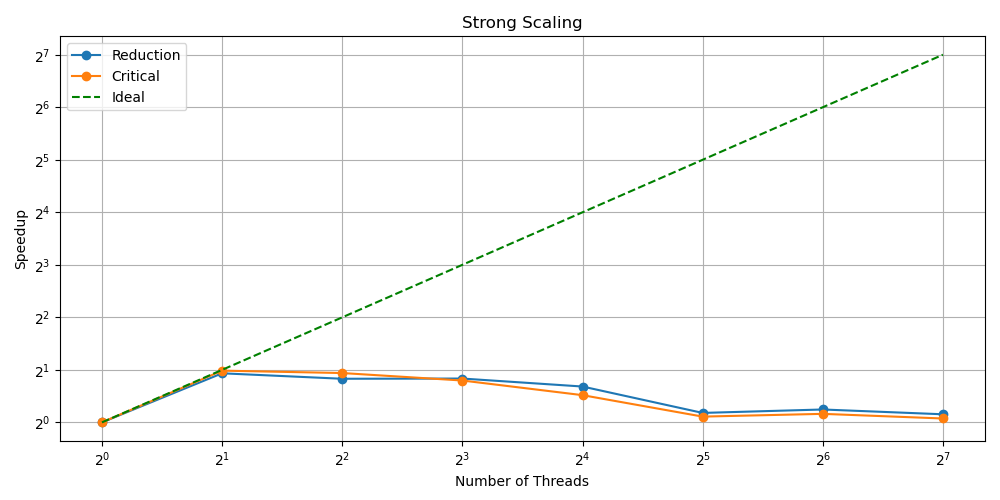
\includegraphics[width=0.8\textwidth]{../pi/strong_scaling_plot.png}
      \caption{Strong scaling efficiency}
      \label{fig:strong-scaling}
    \end{figure}
    From the figure, we can see that the efficiency of the parallel code with
    the reduction clause is quite similar than that with the critical directive.
    The analysis was done taking the mean of 100 trials for each number of
    threads.
    We can also see that the results are far from the ideal efficiency of slope
    one, but this is expected and often the case for parallelization effforts.
    The discrepancy can be attributed to the overhead of communication and
    synchronization between threads, which is not present in the serial code.
    We could also try making the problem size larger to see if the speedup improves.
    
    If time to solution is not the primary objective because larger problem
    sizes (with limited memory) are of interest, it is appropriate to perform
    what is known as \textbf{weak scaling}. In this analysis, we scale the
    problem size with some power of N and analyze the difference in efficiency.
    We use the following formula to calculate efficiency $E$,
    \begin{align}
      E =  \frac{T(1)}{p*T(N)}.
    \end{align}
    The difference between strong and weak scaling is that in the former the
    problem size is fixed, while in the latter the problem size is scaled with
    the number of workers.
    For our problem, we present the results of the weak scaling efficiency in
    Figure \ref{fig:weak-scaling}.
    \begin{figure}[h]
      \centering
      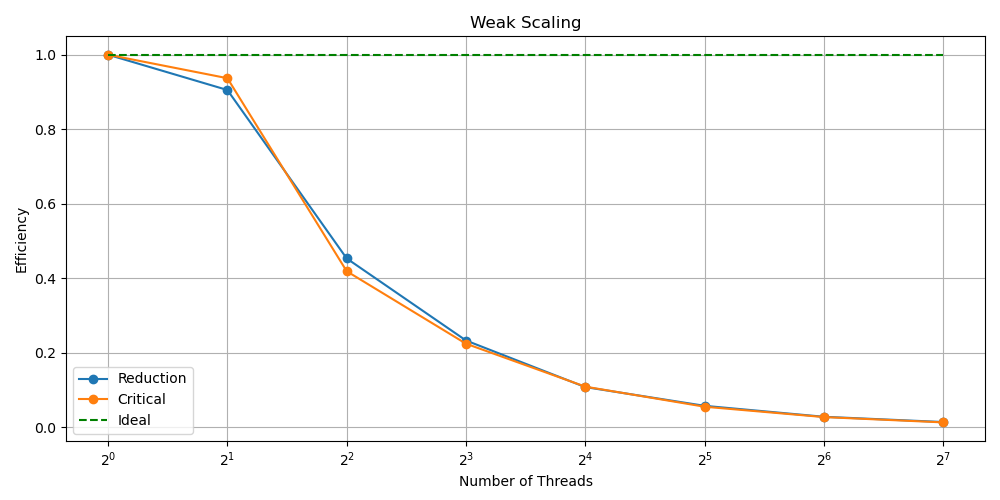
\includegraphics[width=0.8\textwidth]{../pi/weak_scaling_plot.png}
      \caption{Weak scaling efficiency}
      \label{fig:weak-scaling}
    \end{figure}
    Similarly to the strong scaling, we can see that both implementations
    produce similar results. The same arguments can be made for the discrepancy
    between the ideal efficiency and the actual efficiency.

\end{enumerate}

\section{The Mandelbrot set  using \texttt{OpenMP} [20 points]}
This exercise is about parallelizing the computation of the Mandelbrot set using
the \texttt{OpenMP} directive. The Mandelbrot set is a set of complex numbers
$c$ for which the function $f_c(z) = z^2 + c$ does not diverge when iterated
from $z = 0$.
Bellow is the code snippet that shows the sequential implementation on the provided
template.
\begin{cppverbatim}
// do the calculation
cy = MIN_Y;
for (j = 0; j < IMAGE_HEIGHT; j++)
{
  cx = MIN_X;
  for (i = 0; i < IMAGE_WIDTH; i++)
  {
    x = 0;
    y = 0;
    x2 = 0;
    y2 = 0;
    // compute the orbit z, f(z), f^2(z), f^3(z), ...
    // count the iterations until the orbit leaves the circle |z|=2.
    // stop if the number of iterations exceeds the bound MAX_ITERS.
    int n = 0;
    // >>>>>>>>>>>>>>>>>>>>>>>>>>>>>>>>
    while (((x2 + y2) <= 4) & (n < MAX_ITERS))
    {
      y = 2 * x * y + cy;
      x = x2 - y2 + cx;
      x2 = x * x;
      y2 = y * y;
      n++;
      nTotalIterationsCount++;
    }
    // <<<<<<<<<<<<<<<<<<<<<<<<<<<<<<<<
    // n indicates if the point belongs to the mandelbrot set
    // plot the number of iterations at point (i, j)
    int c = ((long)n * 255) / MAX_ITERS;
    png_plot(pPng, i, j, c, c, c);
    cx += fDeltaX;
  }
  cy += fDeltaY;
}
\end{cppverbatim}
The results of the sequential implementation are shown in Figure
\ref{fig:mandelbrot-sequential}. For all calculations, we used the dimensions
$4096\times 4096=16777216$ pixels.
\begin{figure}[h]
  \centering
  
\includegraphics[width=0.5\textwidth]{../mandel/mandel_seq.png}
  \caption{Mandelbrot set sequential implementation}
  \label{fig:mandelbrot-sequential}
\end{figure}
To parallelize code, we can use the \texttt{OpenMP} directive \texttt{parallel
for}. This directive will distribute the iterations of the outer loop among the
threads.
\begin{cppverbatim}
#pragma omp parallel shared(pPng, fDeltaX, fDeltaY, nTotalIterationsCount, num_threads) private(j, i, x, y, y2, x2, cx, cy, n, c)
\end{cppverbatim}
We also add the directive \texttt{\#pragma omp for} for the outer loop.
Other changes include changing the loop index variables to private, and the $cy$
and $cx$, that are the real and imaginary parts of the complex number $c$, to be
calculated from the loop index variables.
\begin{cppverbatim}
cy = fDeltaY * j + MIN_Y;
cx = fDeltaX * i + MIN_X;
\end{cppverbatim}
The resulting image is shown in Figure \ref{fig:mandelbrot-parallel}.
\begin{figure}[h]
  \centering
  
\includegraphics[width=0.5\textwidth]{../mandel/mandel_par.png}
  \caption{Mandelbrot set parallel implementation with 128 threads.}
  \label{fig:mandelbrot-parallel}
\end{figure}
We also performed a strong scaling study of the parallel implementation. The
results are shown in Figure \ref{fig:mandelbrot-strong-scaling}.
\begin{figure}[h]
  \centering
  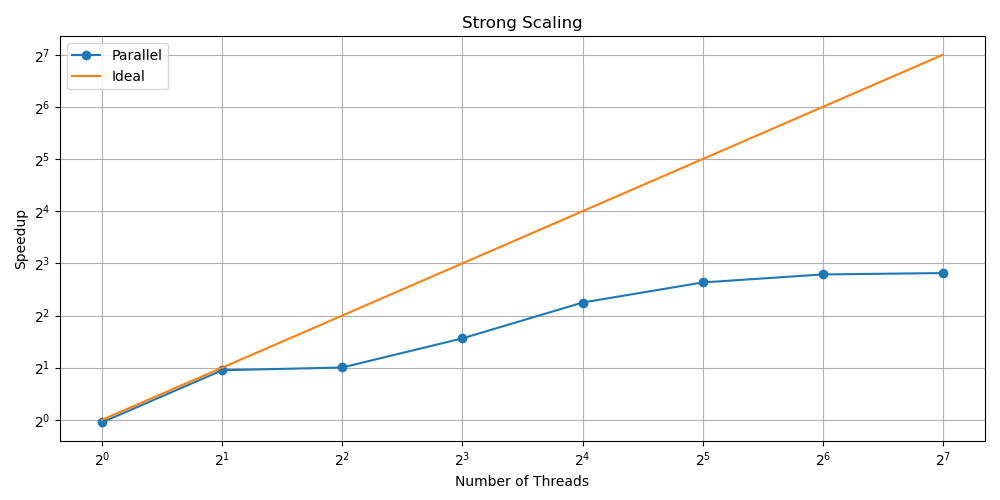
\includegraphics[width=0.8\textwidth]{../mandel/strong_scaling_plot.png}
  \caption{Mandelbrot set strong scaling efficiency}
  \label{fig:mandelbrot-strong-scaling}
\end{figure}

\begin{table}[htbp]
  \centering
  \begin{tabular}{|c|c|c|c|c|c|c|}
  \hline
   Threads & Total time& Avg. time/pixel& Avg. time/iter& Iter/sec & MFlop/s &  N iter\\
  \hline
   Serial & 323.388 & 1.9275E-05 & 2.85E-09 & 3.51E+08 & 2810.86 & 113624527400\\
   1 & 334.444  & 1.9934E-05 & 2.94E-09 & 3.40E+08 & 2718.6 & 113652339001\\
   2 & 167.27  & 9.9700E-06 & 1.47E-09 & 6.79E+08 & 5434.83 & 113635259482\\
   4 & 161.266  & 9.6122E-06 & 1.42E-09 & 7.05E+08 & 5637.06 & 113633417598\\
   8 & 109.512  & 6.5274E-06 & 9.64E-10 & 1.04E+09 & 8300.58 & 113626596677\\
   16 & 68.0375  & 4.0553E-06 & 5.99E-10 & 1.67E+09 & 13355.3 & 113582813215\\
   32 & 52.095  & 3.1051E-06 & 4.59E-10 & 2.18E+09 & 17442.4 & 113582841475\\
   64 & 46.8211  & 2.7907E-06 & 4.12E-10 & 2.43E+09 & 19411 & 113605732438\\
   128 & 45.9884  & 2.7411E-06 & 4.05E-10 & 2.47E+09 & 19762.9 & 113607727564\\
  \hline
  \end{tabular}
  \caption{Performance Metrics. Time is presented in seconds. ``Iter'' is short for iterations.}
  \label{tab:performance_metrics}
  \end{table}

  We can see some discrepancies in the number of iterations for the different
  number of threads. This is some kind of numerical instability or incorrect
  implementation of race conditions. We also see that there are
  more points than there should be on the x-axis that do not appear on the
  sequential implementation. We had a lengthy discussion on
  this issue, but we were not able to find a solution. It may be related to the
  truncation of the floating point numbers.

  On the other hand, we can see that the performance metrics are quite good. The
  number of iterations is quite large and this allows for the parallelization to 
  be effective. We can see that the number of MFlop/s is increasing with the
  number of threads, which is expected and a good sign of strong scaling.

\section{Bug hunt [10 points]}

\begin{enumerate}
  \item \textbf{Bug 1} This code has a compilation error and the output is:
  \begin{grayverbatim}
omp_bug1.c:25:3: error: statement after '#pragma omp parallel for' must be a for loop
  {
  ^
1 error generated.
  \end{grayverbatim}

The error involves a incorrect placing of the \texttt{parallel for} directive.
It must be placed before the for loop but in the code it has an extra line
getting the number of threads before the for loop section starts. The correct
implementation involves moving this line inside the for loop and removing hte
extra curly brackets.

  \item \textbf{Bug 2}
The second code has a bug at runtime. When I change the 
\texttt{OMP\_NUM\_THREADS$=$4} and then run the code, I get this output:
\begin{grayverbatim}
Thread 2 is starting...
Number of threads = 4
Thread 0 is starting...
Thread 1 is starting...
Thread 3 is starting...
Thread 3 is done! Total= 0.000000e+00
\end{grayverbatim}

  The problem is that the \texttt{total} variable is not being updated correctly.
  The solution is to declare the total variable as a shared variable by adding
  \texttt{shared(total)} to the \texttt{parallel} directive. Also the location of
  setting the total to zero must be before the parallel structure starts. SO that
  it is not being reinitialized iwth each thread. Finally,  \texttt{reduction(+ :
  total)} or a similar class is needded to update the total variable correctly.
  Additionally, the print
  statement is only useful if you want to know that the program has ended but not
  for each thread. 

  \item \textbf{Bug 3}
  Code three also has a bug at runtime. The idea behind the code is to perform two
  sections on different threads. When running the program with 2 threads, it
  performs the action and ends the program correctky. However, when running it
  with 4 threads, I get the whole output but then the program hangs.
  What I did was to remove the \texttt{\#pragma omp barrier} directive in the
  function \textbf{print\_results}. This directive is not needed because the
  \texttt{\#pragma omp sections} directive already has a barrier at the end of
  the section. The barrier directive is causing the program to hang because it
  is waiting for all threads to reach the barrier, but it is never
  reached because the program is already done.

  \item \textbf{Bug 4}
  Code number four causes a segmentation fault. Apparently, the error is related
 to a
  memory allocation problem. The solution can be done two ways, by setting the
  \texttt{export OMP\_STACKSIZE="9M"} manually or allocating memory dynamically
  using \texttt{malloc} and \texttt{free}. The second option is the best
  solution because it is more portable and does not depend on the system
  settings, but the first option is also valid and does not require any code
  changes. We choose 9M because we know it is an array of 1048 elements of type
  double, so we need at least $1048*8=8384$ bytes. We add a little more to be
  safe.

  \item \textbf{Bug 5}
  Code number five creates another runtime error that keeps the program hanging.
  The issue appears to be related to the locks set between the threads. The
  error occurs because the locks are not being set and released properly. The
  solution is to set and unset corrsponding lockes referring to the
  initialization of both arrays and then the same but calling for the other
  arrays lock for the addition of both of them. This will prevent the deadlock
  by ensuring that both threads are not waiting indefinitely for each other to
  release locks.
  The implementation of only one section is exemplified below, and the structure
  is the same for the other section, but with the locks inverted.
  \begin{cppverbatim}
#pragma omp section
  {
    printf("Thread %d initializing a[]\n", tid);
    omp_set_lock(&locka);
    for (i = 0; i < N; i++)
      a[i] = i * DELTA;
    printf("Thread %d done with a[]\n", tid);
    omp_unset_lock(&locka);

    omp_set_lock(&lockb);
    printf("Thread %d adding a[] to b[]\n", tid);
    for (i = 0; i < N; i++)
      b[i] += a[i];
    omp_unset_lock(&lockb);
    printf("Thread %d done adding a[] to b[]\n", tid);
  }
  \end{cppverbatim}

\end{enumerate}

\section{Parallel histogram calculation using \texttt{OpenMP} [15 points]}
In this exercise, we will parallelize the computation of a histogram using the
\texttt{OpenMP} directive. The parallelization inlcudes an adaptation of the
logic behind a serial implementation to have a private copy of the histogram for
each thread. The private copies are then combined into a shared histogram at the
end of the parallel region. The code snippet below shows the parallel
implementation of the histogram calculation.
\begin{cppverbatim}
#pragma omp parallel shared(num_threads, dist)
{
  num_threads = omp_get_num_threads();
  // Private copy for each thread
  long private_dist[BINS] = {0}; 

#pragma omp for
  for (long i = 0; i < VEC_SIZE; ++i)
  {
    private_dist[vec[i]]++;
  }

  // Combine private_dist arrays into dist
  for (int i = 0; i < BINS; ++i)
  {
#pragma omp atomic
    dist[i] += private_dist[i];
  }
}
\end{cppverbatim}
Reported are the runtimes of the original (serial) code, as well as the 1-thread
and N-thread parallel implementations. The results are shown in Table
\ref{tab:histogram-runtimes}.
\begin{table}[htbp]
  \centering
  \begin{tabular}{|c|c|}
  \hline
   Threads & Runtime (s)\\
  \hline
  Serial & 1.50307 \\
   1 & 2.81964 \\
   2 & 1.94883 \\
   4 & 0.882659 \\
   8 & 0.543278 \\
   16 & 0.65781 \\
   32 & 0.279733 \\
   64 & 0.19542 \\
   128 & 0.21948 \\
  \hline
  \end{tabular}
  \caption{Runtimes of the original (serial) code, as well as the 1-thread and N-thread parallel implementations.}
  \label{tab:histogram-runtimes}
\end{table}

The results of the strong scaling of the parallel implementation are shown in
Figure \ref{fig:histogram-strong-scaling}.
\begin{figure}[h]
  \centering
  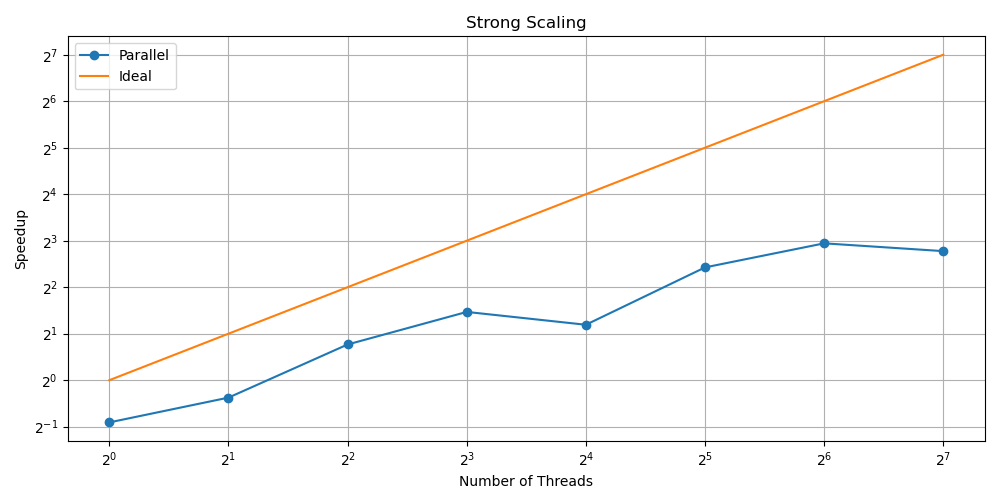
\includegraphics[width=0.8\textwidth]{../hist/strong_scaling_plot.png}
  \caption{Histogram calculation strong scaling efficiency}
  \label{fig:histogram-strong-scaling}
\end{figure}
From the results, we can see that the parallel implementation is not as
efficient for the 1-thread case as the serial implementation. This is expected
because of the change in logic using creating a private data structure for each
independent thread. However, the parallel implementation
becomes more efficient for the 4-thread case and beyond. The serial
case is by itself a good implmentation due to the small problem size, and the
use of optimization flags in the compilation of the code. We can argue that as
the problem size increases, the parallel implementation will be more efficient
than the serial implementation. Additionally, only one run was performed for
each number of threads, so the results may not be very accurate. More runs would
be beneficial to get a better idea of the efficiency of the serial and parallel code.

\section{Parallel loop dependencies with \texttt{OpenMP} [15 points]}
This exercise is about parallelizing a loop with dependencies using the
\texttt{firstprivate} and \texttt{lastprivate}. The trick behind this exercise
is to introduce the power function to calculate the Sn value at the begining of
each iteration. The code snippet below shows the parallel implementation of the
loop with dependencies.
\begin{cppverbatim}
#pragma omp parallel shared(opt, N, up) private(n, i)
{
  i = 0;
#pragma omp for firstprivate(Sn) lastprivate(Sn)
  for (n = 0; n <= N; ++n)
  {
    if (i == 0)
    {
      Sn = Sn * pow(up, n);
      i += 1;
    }
    opt[n] = Sn;
    Sn *= up;
  }
}
\end{cppverbatim}
The Table \ref{tab:parallel-results} shows the results of the
parallel implementation in terms of the runtimes as well as the final result of
the $Sn$ value and the squared norm of the $opt$ vector.
\begin{table}[h]
    \centering
    \begin{tabular}{|c|c|c|c|}
    \hline
    Threads & Parallel Runtime & Final Result $Sn$ & Result $||opt||^2_2$ \\
    \hline
    Serial & 8.232878 & 485165097.62511122 & 5884629305179574 \\
    1 & 8.144716 & 485165097.62511122 & 5884629305179574 \\
    2 & 4.018959 & 485165097.62535083 & 5884629305185405 \\
    4 & 2.301102 & 485165097.62508273 & 5884629305178888 \\
    8 & 1.933245 & 485165097.62554055 & 5884629305189930 \\
    16 & 1.392649 & 485165097.62517869 & 5884629305181860 \\
    32 & 1.173677 & 485165097.62515235 & 5884629305181374 \\
    64 & 1.332998 & 485165097.62513387 & 5884629305180411 \\
    128 & 1.109134 & 485165097.62501615 & 5884629305179745 \\
    \hline
    \end{tabular}
    \caption{Parallel Runtimes and Results. The time is shown in seconds.}
    \label{tab:parallel-results}
\end{table}
The results are quite
similar but we can see some discrepancies in the results. These can be
attributed to the floating point arithmetic and the parallelization of the code.
The results of the strong scaling of the parallel implementation are shown in Figure
\ref{fig:loop-dependencies}.
\begin{figure}[h]
  \centering
  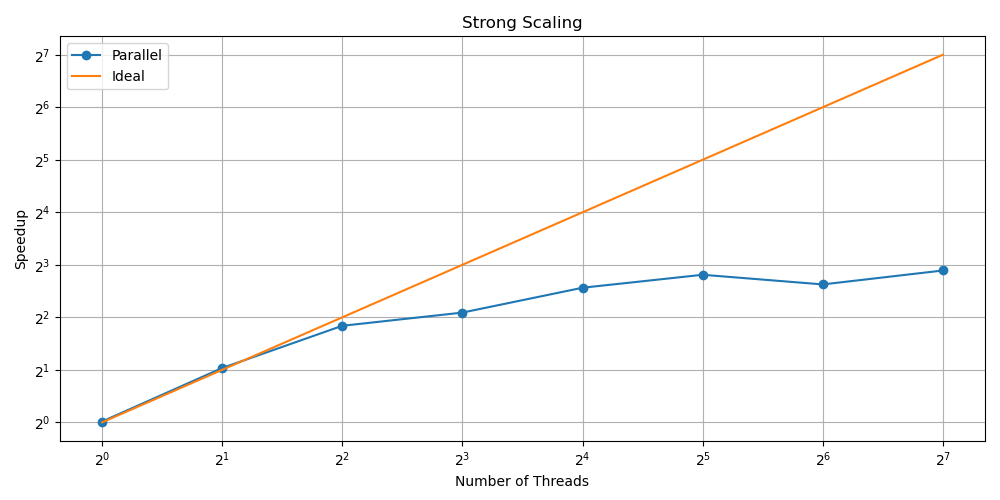
\includegraphics[width=0.8\textwidth]{../loop-dependencies/strong_scaling_plot.png}
  \caption{Loop dependencies strong scaling efficiency}
  \label{fig:loop-dependencies}
\end{figure}
We can see that the parallel implementation is quite efficient in reducing the
total runtime of the code and follows an expected trend common in parallel 
computing.
\section{Quicksort using \texttt{OpenMP} tasks [20 points]}
The final task of the report involves parallelizing the quicksort algorithm
using the \texttt{OpenMP} tasks directive. For my implementation, I used the
\texttt{task} directive to create tasks for the recursive calls of the
quicksort. I also used the \texttt{single} directive to create a single task 
per thread to handle the partitioning of the array. The code snippets below
shows the parallel implementation of the quicksort algorithm.
\begin{cppverbatim}
#pragma omp task
  quicksort(data, right);
#pragma omp task
  quicksort(&(data[left]), length - left);
\end{cppverbatim}

\begin{cppverbatim}
#pragma omp parallel
#pragma omp single
quicksort(data, length);
\end{cppverbatim}
Figure \ref{fig:quicksort} shows the results of the strong scaling of the
parallel implementation of the quicksort algorithm for different array sizes.
\begin{figure}[h]
  \centering
  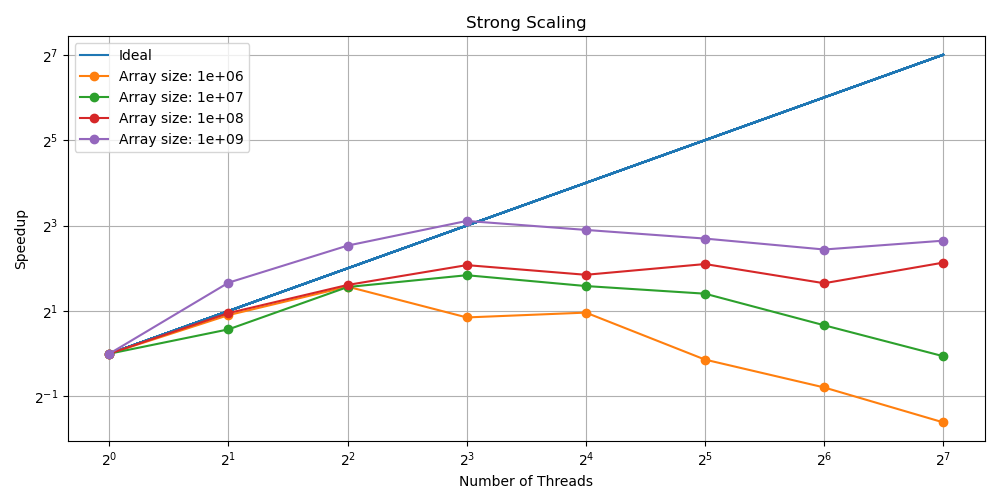
\includegraphics[width=0.8\textwidth]{../quicksort/strong_scaling_plot.png}
  \caption{Quicksort parallel implementation}
  \label{fig:quicksort}
\end{figure}
We can see some interesting results for the different sizes, but the general
trend is that the parallel implementation works well on the lower number of
threads than on the higher number of threads. The
implementation is quite efficient for the smaller array sizes, but it seems to
be even better for the larger array sizes. 
This is expected because the larger array sizes require more work to be done per
thread.
We can also see an improvement beyond the ideal line on the largest array size, $1e+09$, but
we can argue that since this was only analyized over one run, that the time may not be very
accurate.
For the smaller array size, we can see that the parallel implementation becomes
less efficient as the number of threads increases, even less efficient than the
run on a single thread in some cases.
A good consideration to take into account is that the code is the recursive
nature of the algorithm; the work that is done in the last levels of the recursion is very
small, and therefore using so many threads is not beneficial. The overhead of
synchronization and communication between threads is not worth the small amount
of work that is done.
This is why we see
the results for the larger array sizes not being as good as for the smaller
array sizes.
In conclusion, the results are quite good and show that the
parallel implementation is quite efficient in reducing the total runtime of the
code for a limited number of threads, reaching results close to ideal up to 8
threads.

\bibliographystyle{plain}
\bibliography{refs} % Entries are in the refs.bib file

\end{document}
